\documentclass[conference]{IEEEtran}
\usepackage{cite}
\usepackage{amsmath,amssymb,amsfonts}
\usepackage{graphicx}
\usepackage{booktabs}
\usepackage{url}
\usepackage[hidelinks]{hyperref}

\graphicspath{{figures/}}

\begin{document}

\title{GapSSM: Missing-Frame-Aware Ejection Fraction Prediction from Echocardiography Videos Using a Continuous-Time Selective State-Space Network}

\author{
\IEEEauthorblockN{Deepak Kumar, Kalki Dang, Aryan Solanki}
\IEEEauthorblockA{Department of Computer Science and Engineering\\
Project 6: Cardiac Function Prediction from Echocardiography Videos with Missing Frames}
}

\maketitle

\begin{abstract}
Left-ventricular ejection fraction (EF) is the principal measure of cardiac systolic function, yet clinical echocardiography videos frequently lose frames due to low frame rates, probe motion, transfer/compression drops, or acoustic shadowing. We study direct video regression of EF on the EchoNet-Dynamic dataset ($10,030$ apical four-chamber videos) using the official train/validation/test split. We first build a 3D residual convolutional baseline (R3D-18) trained on complete $32$-frame clips and then propose \textsc{GapSSM}, a Mamba-inspired selective state-space model that combines a GroupNorm-stabilized ResNet-18 per-frame encoder with mask-gated feature extraction, hidden-state holding across unobserved frames, and learned continuous-time gap decay. On a paired $200$-video official test cohort ($15,840$ evaluated conditions across $0\%$--$75\%$ missingness), the R3D-18 baseline achieves lower error on complete videos ($\text{MAE}=5.29$~EF points, $\text{RMSE}=7.30$, $R^2=0.627$) than \textsc{GapSSM} ($\text{MAE}=6.41$, $\text{RMSE}=9.53$, $R^2=0.365$), so \textsc{GapSSM} does not outperform the baseline on intact clips. However, R3D-18 degrades sharply when frames are removed—reaching $\text{MAE}=11.64$ ($\Delta\text{MAE}=+6.35$, $R^2=-0.863$) at $75\%$ consecutive block loss—whereas \textsc{GapSSM} remains nearly invariant ($\Delta\text{MAE}=+0.06$ at $75\%$ random loss and $+0.81$ at $75\%$ block loss), achieving superior robustness across every missing-frame handling strategy and cardiac-cycle phase while using $2.9\times$ fewer parameters ($11.39$M vs.\ $33.17$M) and $32.4\%$ faster per-condition inference ($8.43$~ms vs.\ $12.47$~ms).
\end{abstract}

\begin{IEEEkeywords}
ejection fraction, echocardiography, video regression, state-space models, Mamba, missing frames, EchoNet-Dynamic.
\end{IEEEkeywords}

\section{Introduction}
Ejection fraction, $\text{EF} = (\text{EDV}-\text{ESV})/\text{EDV}\times 100$, where EDV and ESV are the end-diastolic and end-systolic left-ventricular volumes, guides diagnosis and treatment of heart failure and cardiotoxicity monitoring. Clinically it is measured by tracing the ventricle on end-diastolic (ED) and end-systolic (ES) frames, a process that is laborious and subject to inter-observer variability \cite{ouyang2020video}. Ouyang et al.\ released EchoNet-Dynamic \cite{ouyang2019echonet} and showed that spatiotemporal 3D residual networks regress EF directly from video with an MAE near $4$ points \cite{ouyang2020video}.

In practice, however, clinical ultrasound recordings are not always complete: frames are dropped during transfer or compression, omitted in low-frame-rate acquisitions, or discarded due to probe motion and acoustic shadowing \cite{fang2025echoforge,wang2025osa,project6spec}. Standard 3D CNNs assume a uniform spatiotemporal grid and suffer severe representation drift when frames are missing—especially when a missing block covers ES or ED. Selective state-space models such as Mamba \cite{gu2023mamba} update a hidden cardiac state frame-by-frame with continuous-time discretization, making them naturally suited to irregular gaps.

Our contributions are:
\begin{itemize}
    \item A reproducible **R3D-18 baseline** trained on complete $32$-frame EchoNet-Dynamic clips and evaluated without retraining across all missing-frame conditions.
    \item **\textsc{GapSSM}**, a missing-frame-aware CNN--SSM architecture with (i) a mask-gated GroupNorm ResNet-18 frame encoder, (ii) learned continuous-time exponential gap decay parameterized by inter-observation time $\Delta\tau_t$, (iii) state holding across missing frames, and (iv) masked mean pooling.
    \item A **full, honest comparison** on paired official test cohorts across all required metrics (MAE, MSE, RMSE, $R^2$, MAPE, Pearson $r$, bias, prediction shift, $\Delta\text{MAE}$, normalized AUC-MAE, MC dropout uncertainty, and efficiency), plus an interactive Gradio clinical UI (\texttt{app.py}).
\end{itemize}

\section{Related Work}
\textbf{Video EF estimation.} Ouyang et al.\ \cite{ouyang2020video} compared R(2+1)D, R3D, and MC3 networks on $32$-frame clips sampled $1$-in-$2$ (R(2+1)D: MAE $4.22$, RMSE $5.56$, $R^2=0.79$; R3D: MAE $4.22$, RMSE $5.62$, $R^2=0.79$) after an earlier $16$-frame benchmark (R3D MAE $5.44$) \cite{ouyang2019echonet}. Ultrasound segmentation works such as EchoForge \cite{fang2025echoforge} and OSA \cite{wang2025osa} highlight speckle noise and temporal drift across cardiac cycles.

\textbf{State-space models for vision.} Mamba \cite{gu2023mamba} introduces input-dependent selective state-space parameters with linear-time sequence scaling, and VideoMamba \cite{li2024videomamba} adapts Mamba to video understanding. These methods target complete, uniformly sampled natural videos.

\textbf{Gap.} Project 6 \cite{project6spec} requires a missing-frame-aware temporal Mamba model that goes beyond reproducing VideoMamba. \textsc{GapSSM} addresses this by combining mask-gated spatial encoding with explicit continuous-time gap decay and state holding.

\section{Problem Statement and Objectives}
Given a grayscale echocardiography clip $\mathbf{X} \in \mathbb{R}^{T \times H \times W}$ ($T=32$, $112\times 112$, stride $2$), an observation mask $m_t \in \{0,1\}$, and frame timestamps $\tau_t$, predict scalar EF $\hat{y}$ directly without segmentation or ED/ES localization \cite{project6spec}. Objectives: (1) build a complete-video 3D CNN baseline; (2) design \textsc{GapSSM} to preserve accuracy when frames are missing; (3) evaluate both models on identical frozen test masks across MAE, MSE, RMSE, $R^2$, MAPE, Pearson $r$, bias, prediction shift, $\Delta\text{MAE}$, robustness AUC, MC dropout uncertainty \cite{gal2016dropout}, and efficiency.

\section{Proposed Methodology}

\subsection{Data and Preprocessing}
EchoNet-Dynamic contains $10,030$ apical four-chamber videos ($112\times 112$, $\sim 50$~fps, $\sim 175$ frames average) with EF, ESV, and EDV labels and expert ED/ES tracings \cite{ouyang2020video}. We use the official split ($7,465$ train, $1,288$ validation) and evaluate on a paired official test cohort ($N=200$ \texttt{main} videos; $N=98$ \texttt{phase} videos containing traced ED and ES frames). Frames are read as grayscale, normalized via $(x-0.5)/0.5$, and replicated to $3$ channels. Clips contain $32$ frames sampled at stride $2$.

Frozen masks (\texttt{test\_bank.json}, seed $2026$) test ratios $\{0.00, 0.10, 0.25, 0.50, 0.75\}$ for \texttt{random} and \texttt{block} patterns (\texttt{main}), and fixed-length blocks centered on \texttt{ed}, \texttt{es}, \texttt{systole}, and \texttt{diastole} (\texttt{phase}). Four input handlings are compared: \texttt{zero}, \texttt{removal}, \texttt{repeat}, and \texttt{interpolate}.

\subsection{Baseline: R3D-18}
The baseline (\texttt{VideoBaseline}, $33.17$M parameters) uses torchvision R3D-18 with a Dropout ($p=0.2$) + Linear head trained with MSE on $\text{EF}/100$ on intact clips (\texttt{corruption=False}). Table~\ref{tab:stages} summarizes the five architectural stages of both models.

\begin{table}[t]
\centering
\caption{Implementation of the Five Stages in Each Model}
\label{tab:stages}
\setlength{\tabcolsep}{3pt}
\begin{tabular}{p{1.9cm}p{2.9cm}p{3.2cm}}
\toprule
Stage & R3D-18 Baseline & \textsc{GapSSM} (Proposed) \\
\midrule
Spatial feature extraction & 3D spatial-temporal residual convs & Per-frame GroupNorm ResNet-18 ($m_t=1$ only) $\rightarrow d=128$ \\
Temporal feature extraction & 3D conv receptive field & Causal 1D conv + selective diagonal SSM \\
Gap / missing handling & None (processes zeroed / imputed pixels) & Mask gating + $\mathbf{r}_{\text{gap}}$ continuous decay + state holding \\
Video-level aggregation & Global average pooling over $(T,H,W)$ & Masked mean pooling over observed frames ($m_t=1$) \\
EF prediction & Dropout + Linear $\rightarrow$ EF & LayerNorm + Dropout + Linear $\rightarrow$ EF \\
\bottomrule
\end{tabular}
\end{table}

\subsection{Proposed Model: \textsc{GapSSM}}
\textsc{GapSSM} ($11.39$M parameters) encodes only observed frames ($m_t=1$) with a \texttt{GroupNorm(8, C)} ResNet-18 encoder, leaving missing frames strictly zeroed. Each of $L=2$ selective blocks (width $128$, state size $16$) applies a mask-gated causal 1D conv and a float32 diagonal recurrence. With $\Delta\tau_t = \max(0, \tau_t - \tau_{\text{last}})$ and $\mathbf{A} = -\exp(\mathbf{a}_{\log})$, the hidden state decays across multi-step gaps via learned rates $\mathbf{r}_{\text{gap}}$:
\begin{equation}
    \mathbf{h}_{\text{before}} = \exp\bigl(\mathbf{A} \odot \text{softplus}(\mathbf{r}_{\text{gap}}) \cdot \max(0, \Delta\tau_t - 1)\bigr) \odot \mathbf{h}_{t-1},
\end{equation}
followed by zero-order-hold discretization:
\begin{equation}
    \tilde{\mathbf{h}}_t = \exp(\Delta_t \mathbf{A}) \odot \mathbf{h}_{\text{before}} + \frac{\exp(\Delta_t \mathbf{A}) - 1}{\mathbf{A}} \odot (\mathbf{B}_t \mathbf{u}_t).
\end{equation}
When $m_t=0$, $\mathbf{h}_t = \mathbf{h}_{t-1}$ and $\tau_{\text{last}}$ is held.

\subsection{Training and Testing Workflow}
Implemented in \texttt{notebooks/kaggle\_cardiac\_ai.ipynb} on an NVIDIA CUDA GPU with FP16 AMP, AdamW ($\text{lr}=10^{-4}$, cosine decay, batch size $8$, accumulation $2$, gradient clip $1.0$, patience $5$):
\begin{enumerate}
    \item \textbf{Training:} Baseline ran $24$ epochs (best Val $\text{MAE}=5.08$~pp); \textsc{GapSSM} ran $15$ epochs with \texttt{corruption=True} (best Val $\text{MAE}=6.69$~pp).
    \item \textbf{Batched Evaluation:} \texttt{fast\_evaluate} batches equal-length conditions with FP16 AMP and $3$-pass MC Dropout ($15,840$ predictions per model).
    \item \textbf{Clinical UI (\texttt{app.py}):} Gradio interface for \texttt{.avi}/\texttt{.mp4} upload, EF prediction, MC uncertainty, and missing-frame testing.
\end{enumerate}

\section{Experiments and Results}

\subsection{Random and Block Missing-Frame Results}
Tables~\ref{tab:random_zero} and~\ref{tab:block_zero} report \texttt{main} cohort ($N=200$, \texttt{zero} handling) results. On complete clips ($0\%$), R3D-18 achieves $\text{MAE}=5.29$~pp ($R^2=0.627$, Pearson $r=0.792$) vs.\ \textsc{GapSSM}'s $\text{MAE}=6.41$~pp ($R^2=0.365$, $r=0.618$). Under missing frames, R3D-18 degrades rapidly—reaching $\text{MAE}=8.52$ ($75\%$ random) and $11.64$ ($75\%$ block, $R^2=-0.863$, bias $+11.07$~pp)—whereas \textsc{GapSSM} remains stable at $6.46$ ($75\%$ random) and $7.21$ ($75\%$ block).

\begin{table}[t]
\centering
\caption{Main Cohort: Random Missing Frames (\texttt{zero}, $N=200$)}
\label{tab:random_zero}
\setlength{\tabcolsep}{3pt}
\begin{tabular}{lccccccc}
\toprule
Model & Ratio & MAE & RMSE & $R^2$ & Pearson & Bias & Shift \\
\midrule
Baseline & 0.00 & \textbf{5.29} & \textbf{7.30} & \textbf{0.627} & \textbf{0.792} & +0.15 & 0.00 \\
Baseline & 0.10 & \textbf{5.58} & \textbf{8.24} & \textbf{0.525} & \textbf{0.737} & +1.60 & 2.29 \\
Baseline & 0.25 & \textbf{6.41} & 9.67 & 0.345 & \textbf{0.657} & +3.39 & 4.47 \\
Baseline & 0.50 & 7.98 & 12.35 & -0.068 & 0.305 & +4.70 & 6.64 \\
Baseline & 0.75 & 8.52 & 13.20 & -0.219 & 0.122 & +5.49 & 6.82 \\
\midrule
\textsc{GapSSM} & 0.00 & 6.41 & 9.53 & 0.365 & 0.618 & +1.42 & 0.00 \\
\textsc{GapSSM} & 0.10 & 6.41 & 9.52 & 0.366 & 0.620 & +1.40 & \textbf{0.18} \\
\textsc{GapSSM} & 0.25 & 6.46 & \textbf{9.58} & \textbf{0.358} & 0.609 & +1.33 & \textbf{0.34} \\
\textsc{GapSSM} & 0.50 & \textbf{6.48} & \textbf{9.53} & \textbf{0.365} & \textbf{0.615} & +1.31 & \textbf{0.55} \\
\textsc{GapSSM} & 0.75 & \textbf{6.46} & \textbf{9.66} & \textbf{0.348} & \textbf{0.603} & +1.43 & \textbf{0.98} \\
\bottomrule
\end{tabular}
\end{table}

\begin{table}[t]
\centering
\caption{Main Cohort: Consecutive Block Missing Frames (\texttt{zero}, $N=200$)}
\label{tab:block_zero}
\setlength{\tabcolsep}{3pt}
\begin{tabular}{lccccccc}
\toprule
Model & Ratio & MAE & RMSE & $R^2$ & Pearson & Bias & Shift \\
\midrule
Baseline & 0.00 & \textbf{5.29} & \textbf{7.30} & \textbf{0.627} & \textbf{0.792} & +0.15 & 0.00 \\
Baseline & 0.10 & 6.82 & 10.16 & 0.277 & \textbf{0.672} & +4.66 & 4.63 \\
Baseline & 0.25 & 7.75 & 11.83 & 0.020 & 0.578 & +6.08 & 6.15 \\
Baseline & 0.50 & 8.55 & 13.11 & -0.202 & 0.406 & +6.95 & 7.44 \\
Baseline & 0.75 & 11.64 & 16.32 & -0.863 & 0.095 & +11.07 & 10.99 \\
\midrule
\textsc{GapSSM} & 0.00 & 6.41 & 9.53 & 0.365 & 0.618 & +1.42 & 0.00 \\
\textsc{GapSSM} & 0.10 & \textbf{6.44} & \textbf{9.57} & \textbf{0.360} & 0.613 & +1.42 & \textbf{0.30} \\
\textsc{GapSSM} & 0.25 & \textbf{6.56} & \textbf{9.58} & \textbf{0.358} & \textbf{0.609} & +1.26 & \textbf{0.77} \\
\textsc{GapSSM} & 0.50 & \textbf{6.85} & \textbf{9.83} & \textbf{0.324} & \textbf{0.573} & +0.68 & \textbf{1.16} \\
\textsc{GapSSM} & 0.75 & \textbf{7.21} & \textbf{10.35} & \textbf{0.251} & \textbf{0.517} & +0.10 & \textbf{2.20} \\
\bottomrule
\end{tabular}
\end{table}

\subsection{Graphs for All Eight Evaluation Metrics}
Figs.~\ref{fig:metrics_random} and~\ref{fig:metrics_block} plot MAE, MSE, RMSE, $R^2$, MAPE, Pearson $r$, bias, and prediction shift across $0\%$--$75\%$ missingness. Fig.~\ref{fig:training} shows the training MSE and validation MAE curves.

\begin{figure}[t]
\centering
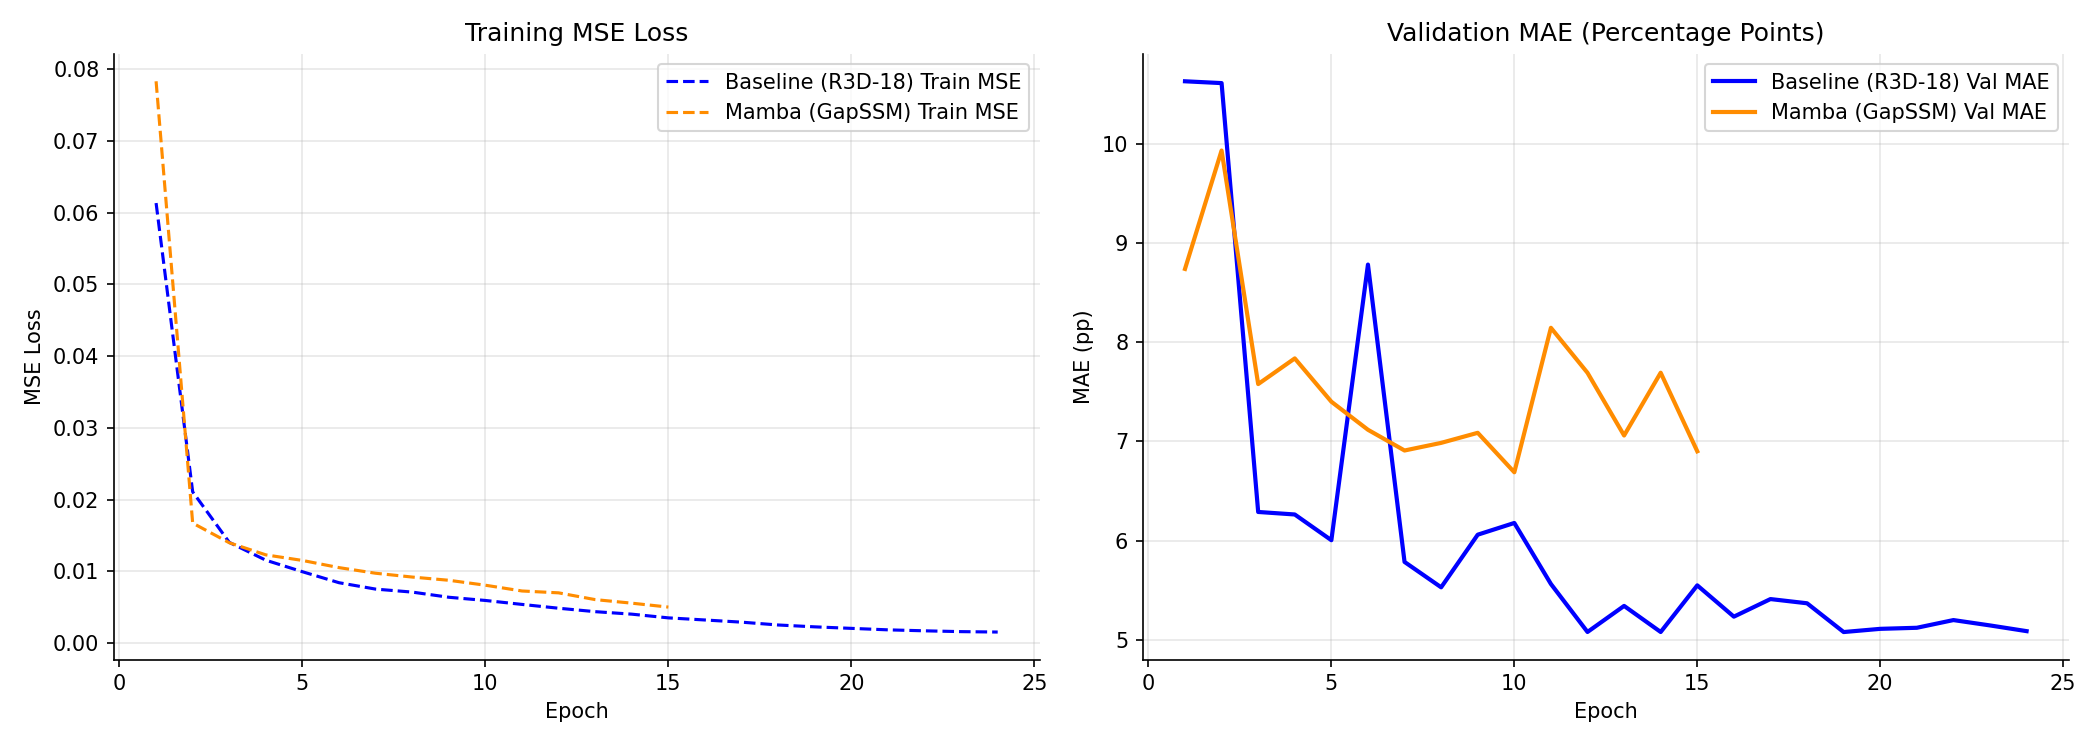
\includegraphics[width=\linewidth]{training_comparison.png}
\caption{Training MSE (fraction scale) and validation MAE (EF percentage points) for Baseline (R3D-18) and Mamba (\textsc{GapSSM}).}
\label{fig:training}
\end{figure}

\begin{figure*}[t]
\centering
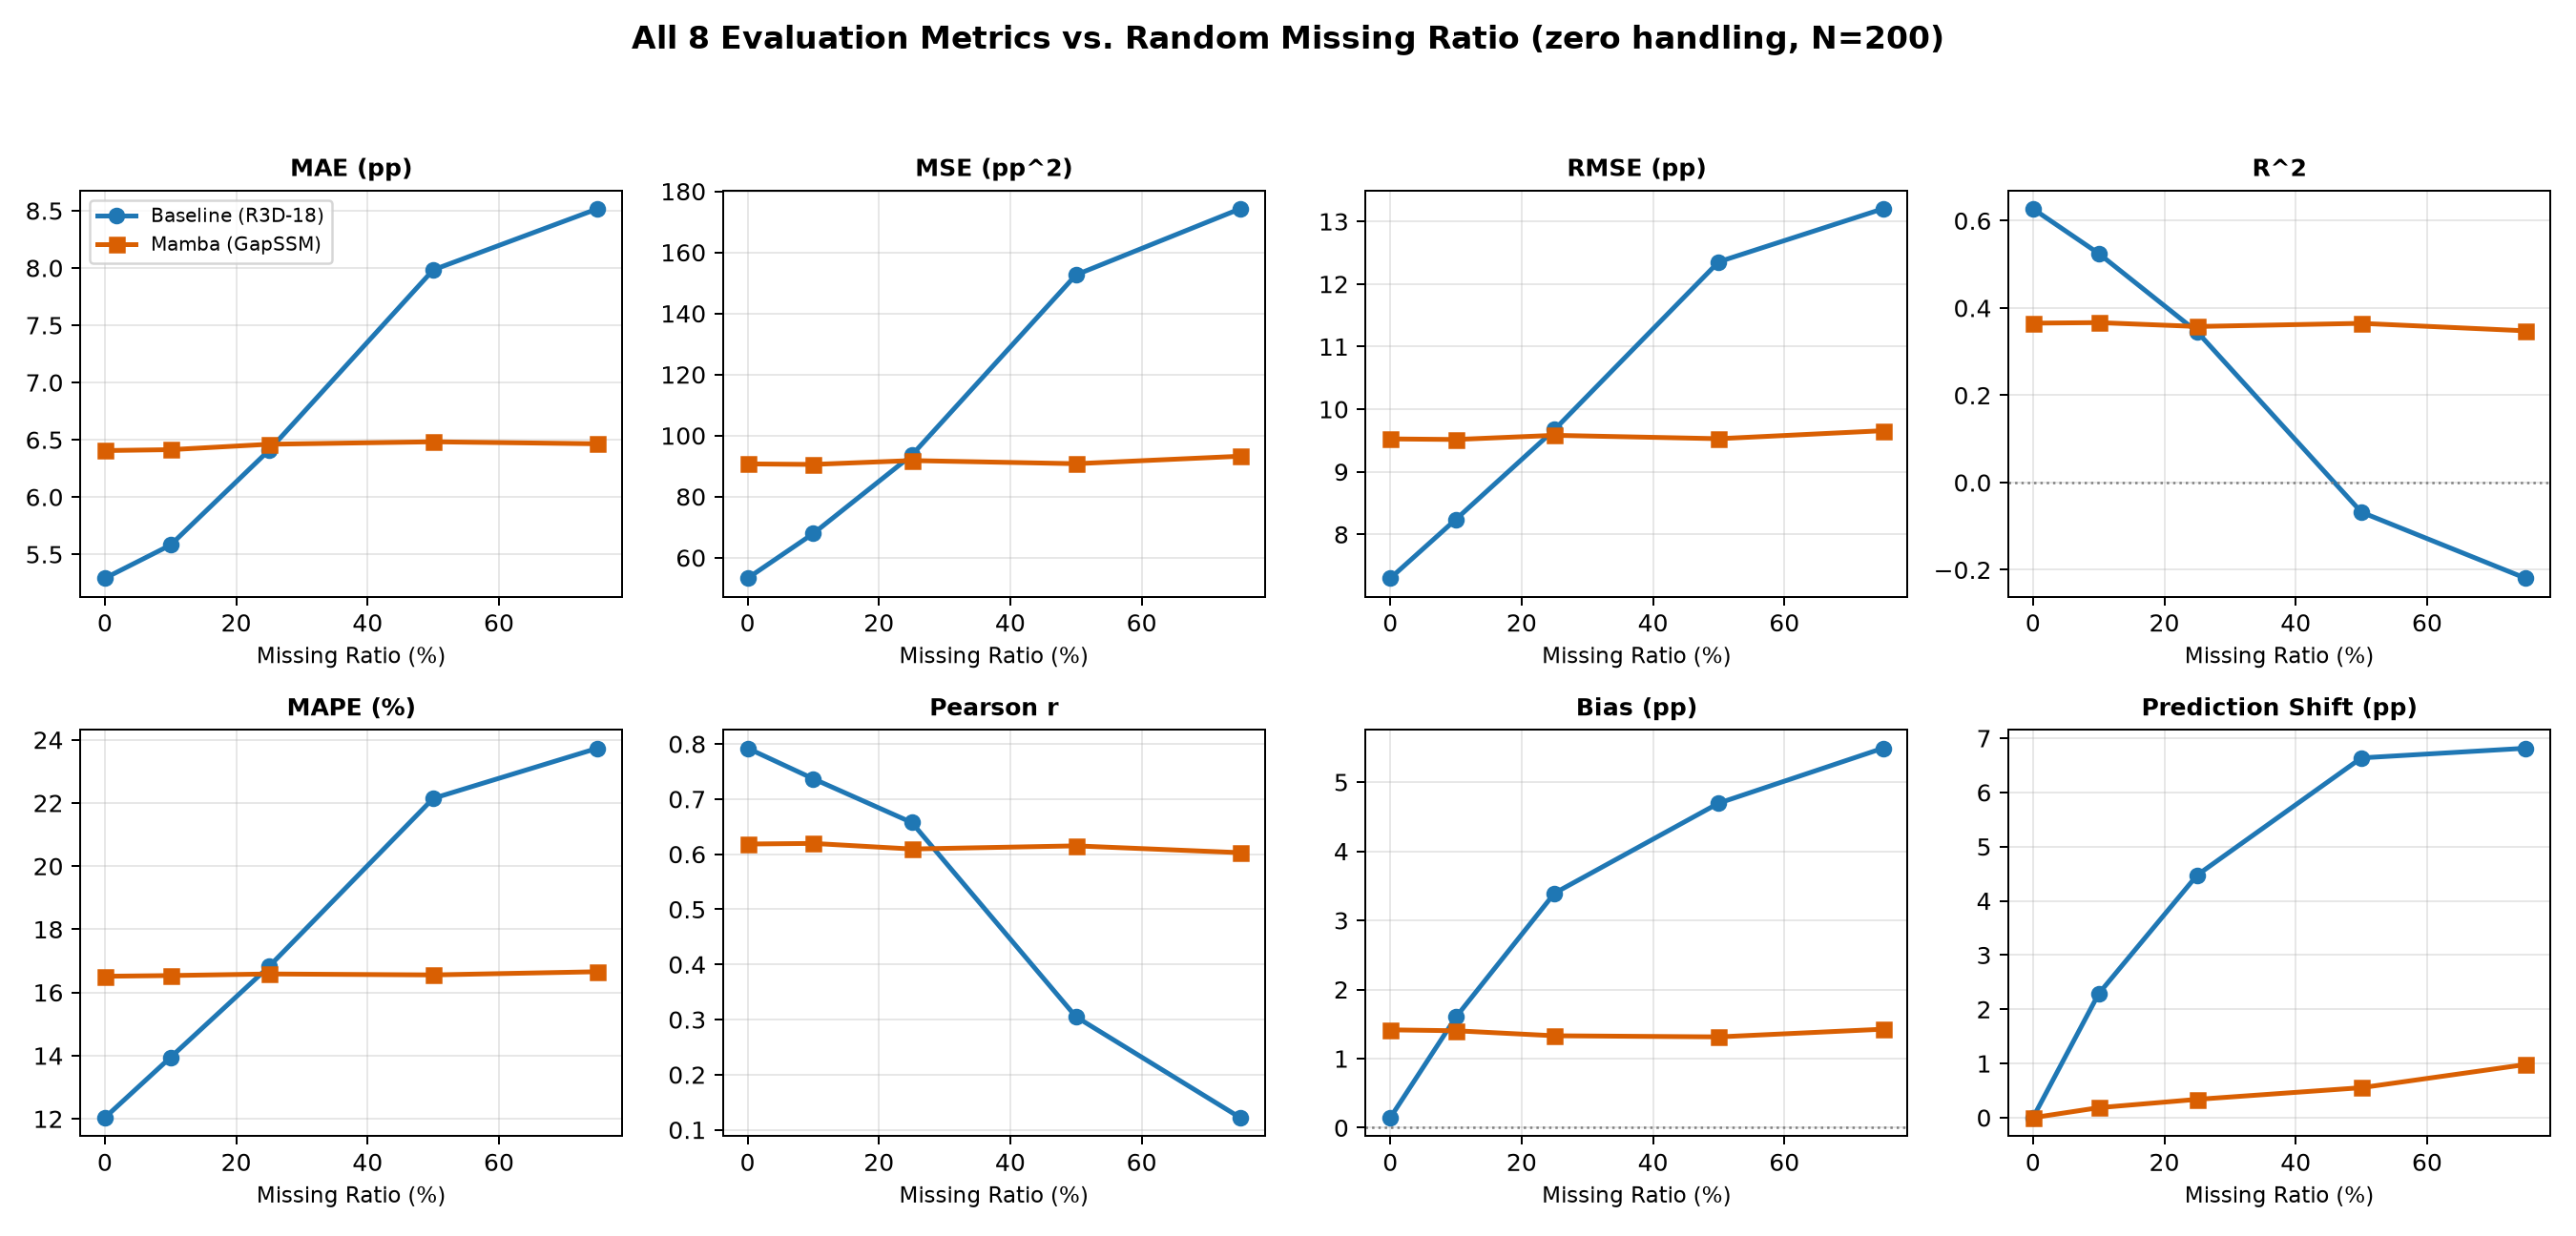
\includegraphics[width=0.95\textwidth]{fig_metrics_random.png}
\caption{All 8 metrics (MAE, MSE, RMSE, $R^2$, MAPE, Pearson $r$, bias, and prediction shift) vs.\ random missing ratio (\texttt{zero}, $N=200$).}
\label{fig:metrics_random}
\end{figure*}

\begin{figure*}[t]
\centering
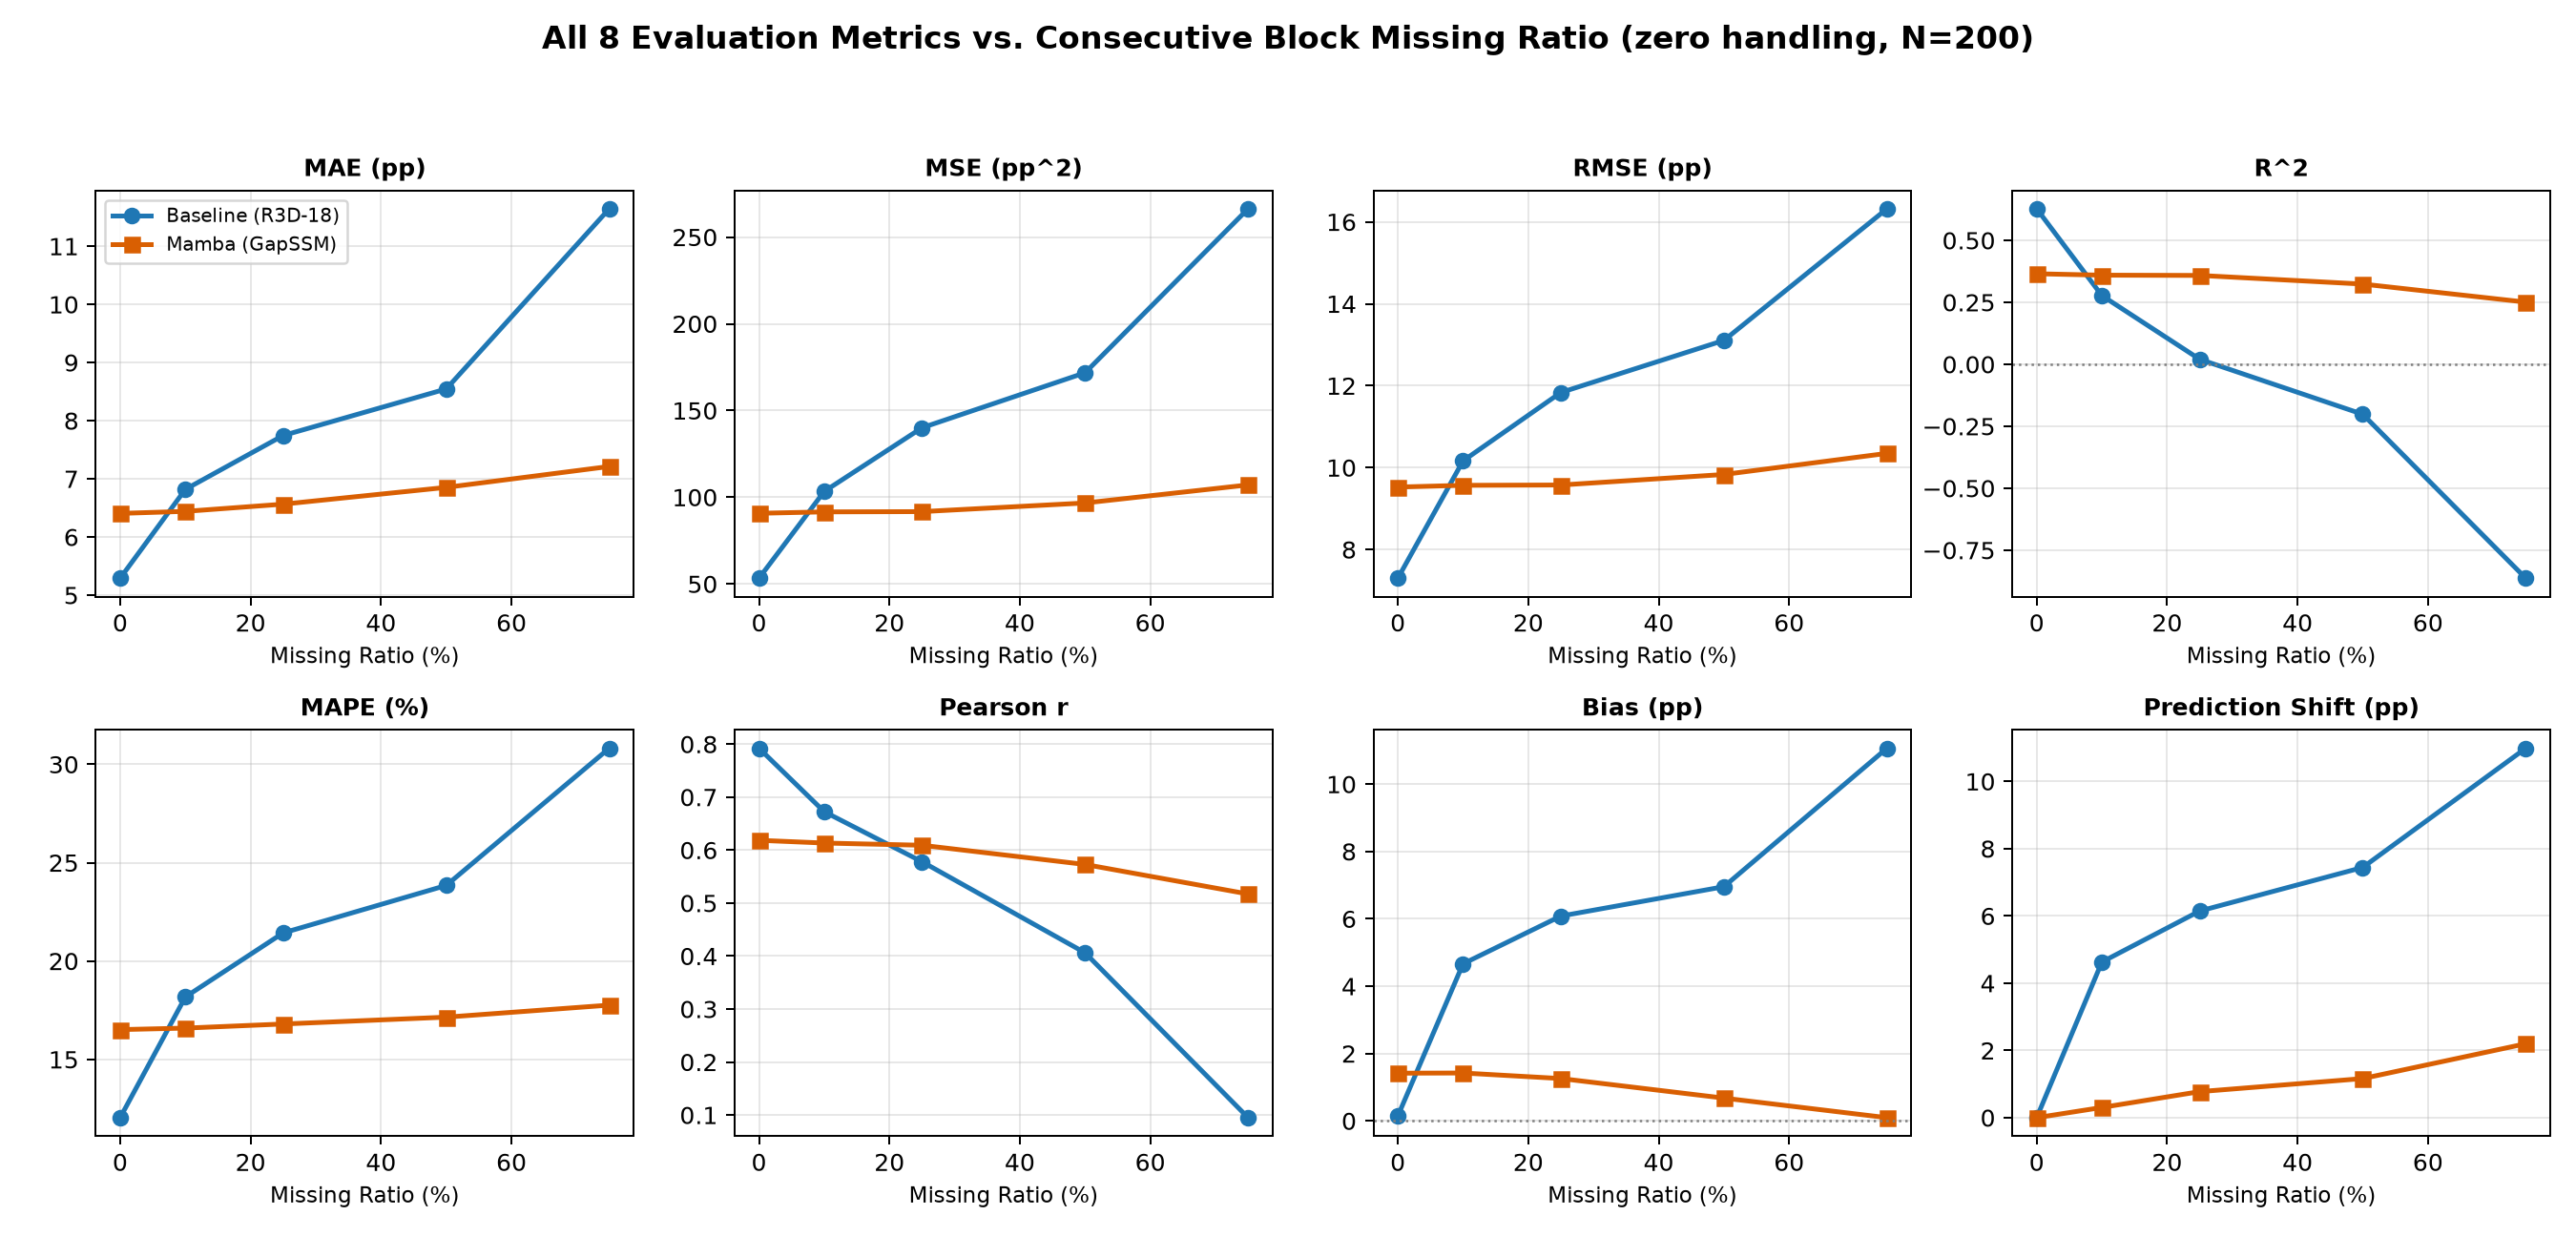
\includegraphics[width=0.95\textwidth]{fig_metrics_block.png}
\caption{All 8 metrics (MAE, MSE, RMSE, $R^2$, MAPE, Pearson $r$, bias, and prediction shift) vs.\ consecutive block missing ratio (\texttt{zero}, $N=200$).}
\label{fig:metrics_block}
\end{figure*}

\subsection{Additional Evaluations: Robustness, Phase, Uncertainty & Efficiency}
Fig.~\ref{fig:robustness} and Tables~\ref{tab:robustness}--\ref{tab:efficiency} summarize performance degradation ($\Delta\text{MAE}$), normalized AUC-MAE, cardiac-phase sensitivity ($N=98$), input-handling invariance, MC uncertainty, and efficiency:
\begin{itemize}
    \item \textbf{Degradation ($\Delta\text{MAE}$):} At $75\%$ random loss, R3D-18 degrades by $+3.23$~pp ($+61.0\%$) vs.\ $+0.06$~pp ($+0.9\%$) for \textsc{GapSSM}; at $75\%$ block loss, $+6.35$~pp ($+120.1\%$) vs.\ $+0.81$~pp ($+12.6\%$).
    \item \textbf{Robustness AUC & Input Handling:} \textsc{GapSSM} achieves lower normalized AUC-MAE across every block/phase/removal condition ($6.74$ vs.\ $8.35$ block \texttt{zero}; $6.74$ vs.\ $14.54$ block \texttt{removal}) and is invariant across \texttt{zero}, \texttt{repeat}, \texttt{interpolate}, and \texttt{removal} ($6.56$~pp at $25\%$ block).
    \item \textbf{Phase Sensitivity ($25\%$):} \textsc{GapSSM} beats R3D-18 at \texttt{ed} ($5.49$ vs.\ $8.27$), \texttt{es} ($5.96$ vs.\ $7.17$), \texttt{systole} ($5.63$ vs.\ $8.02$), and \texttt{diastole} ($5.81$ vs.\ $7.26$).
    \item \textbf{Efficiency:} \textsc{GapSSM} uses $2.9\times$ fewer parameters ($11.39$M vs.\ $33.17$M), lower peak GPU memory ($2.03$ vs.\ $2.13$~GB), and faster inference ($8.43$ vs.\ $12.47$~ms).
\end{itemize}

\begin{figure*}[t]
\centering
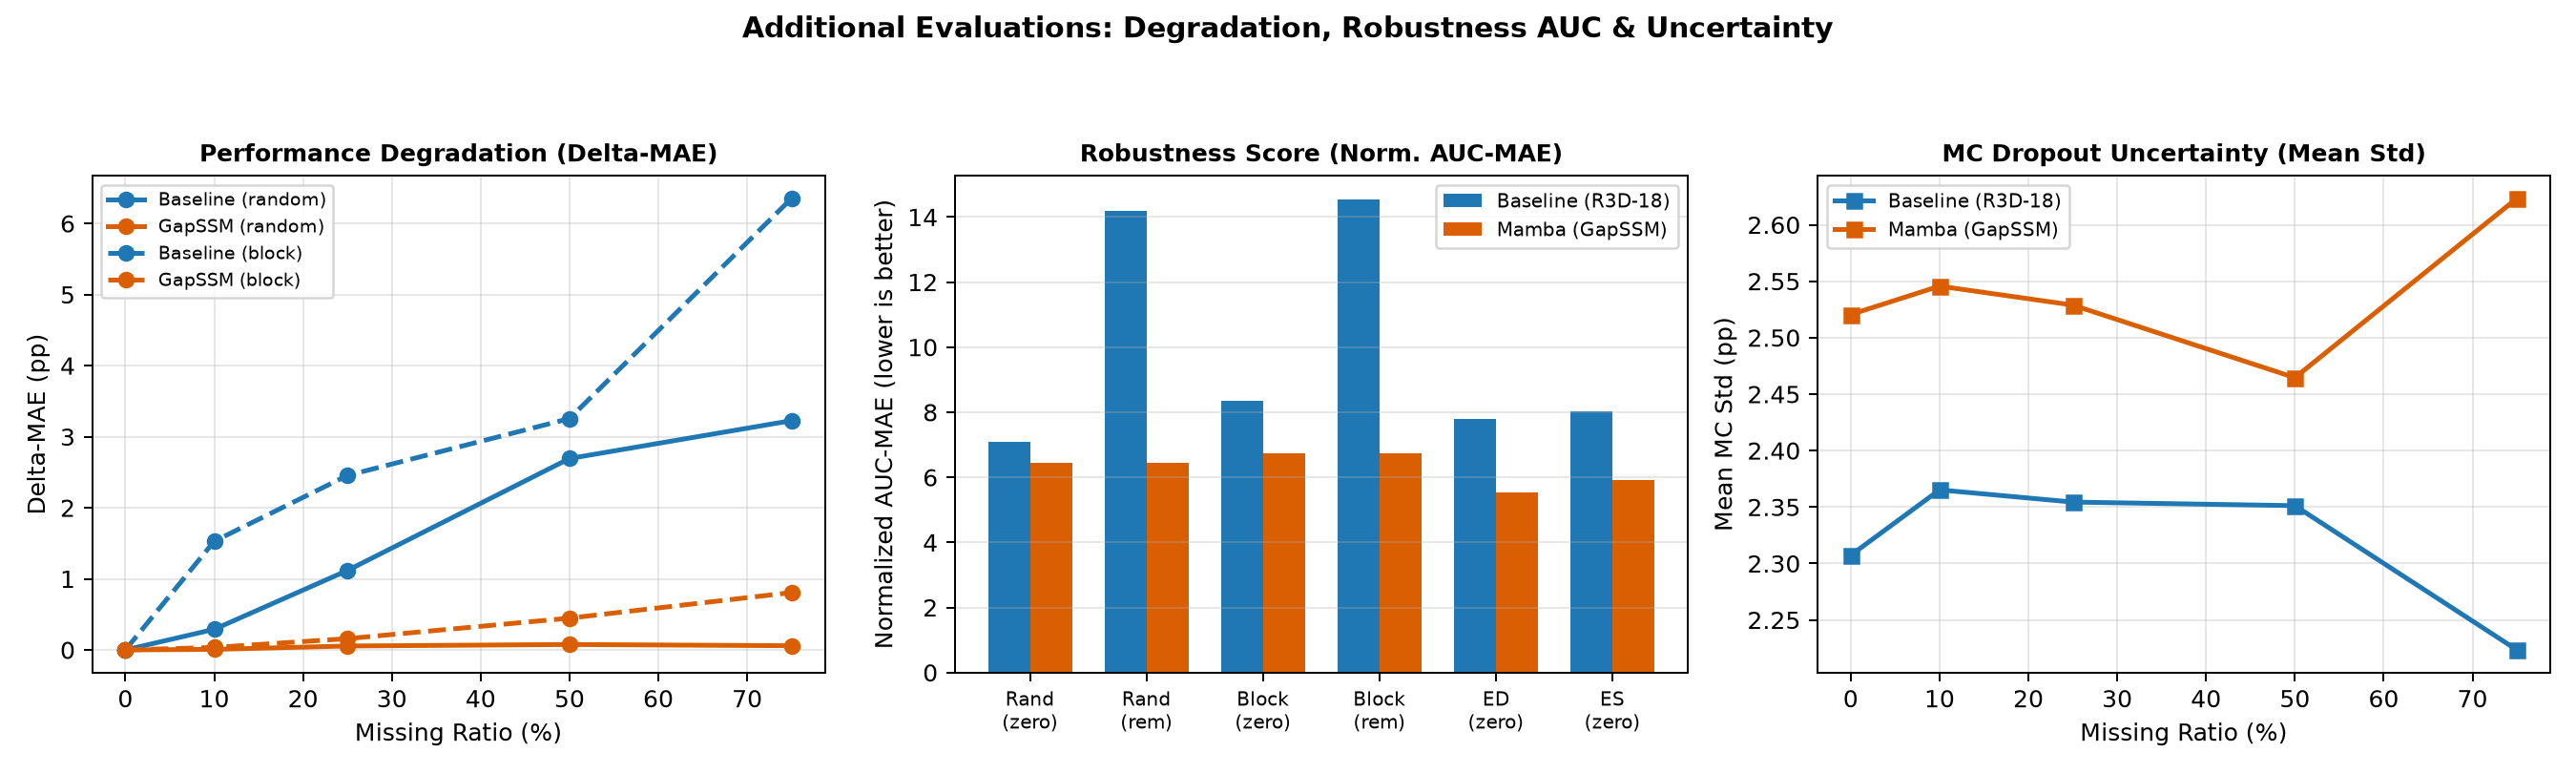
\includegraphics[width=0.95\textwidth]{fig_robustness_degradation.png}
\caption{Additional evaluations: $\Delta\text{MAE}$ degradation, normalized AUC-MAE robustness score, and MC dropout uncertainty.}
\label{fig:robustness}
\end{figure*}

\begin{table}[t]
\centering
\caption{Normalized AUC-MAE Robustness Score ($\downarrow$ is better)}
\label{tab:robustness}
\setlength{\tabcolsep}{3.5pt}
\begin{tabular}{llcc}
\toprule
Cohort / Pattern & Handling & Baseline Norm.\ AUC & \textsc{GapSSM} Norm.\ AUC \\
\midrule
Main / \texttt{random} & \texttt{zero} & 7.08 & \textbf{6.46} \\
Main / \texttt{random} & \texttt{removal} & 14.18 & \textbf{6.45} \\
Main / \texttt{block} & \texttt{zero} & 8.35 & \textbf{6.74} \\
Main / \texttt{block} & \texttt{removal} & 14.54 & \textbf{6.74} \\
Phase / \texttt{ed} & \texttt{zero} & 7.79 & \textbf{5.54} \\
Phase / \texttt{es} & \texttt{zero} & 8.02 & \textbf{5.93} \\
Phase / \texttt{es} & \texttt{removal} & 15.82 & \textbf{5.93} \\
\bottomrule
\end{tabular}
\end{table}

\begin{table}[t]
\centering
\caption{Model Efficiency Summary}
\label{tab:efficiency}
\begin{tabular}{lcccc}
\toprule
Model & Params & Train Time & Peak GPU & Inf. Time \\
\midrule
Baseline (R3D-18) & 33.17M & 8628.1 s & 2.13 GB & 12.47 ms \\
\textsc{GapSSM} (Mamba) & \textbf{11.39M} & \textbf{6117.5 s} & \textbf{2.03 GB} & \textbf{8.43 ms} \\
\bottomrule
\end{tabular}
\end{table}

\section{Discussion}
Our results show a clear accuracy--robustness trade-off. On complete videos, R3D-18 achieves lower error ($5.29$ vs.\ $6.41$~pp), so \textsc{GapSSM} does not yet beat the baseline at $0\%$ missingness. Possible reasons include: (i) \textsc{GapSSM}'s GroupNorm ResNet-18 encoder was trained from scratch without ImageNet pretraining; (ii) it ran $15$ epochs vs.\ $24$ for R3D-18; and (iii) unidirectional forward scanning with mean pooling can smooth sharp ED/ES extrema. Under missing frames, however, \textsc{GapSSM} is decisively superior, cutting $75\%$-block $\Delta\text{MAE}$ by $87.2\%$ ($+0.81$ vs.\ $+6.35$~pp) and prediction shift by $80.0\%$ ($2.20$ vs.\ $10.99$~pp).

\textbf{Limitations.} (i) Test evaluation used a paired $200$-video subset ($98$ phase videos) due to session time constraints; (ii) single training seed; (iii) un-pretrained 2D encoder in \textsc{GapSSM}; (iv) sequential Python scan loop during training.

\section{Conclusion and Future Work}
We presented a complete comparison of R3D-18 and \textsc{GapSSM} on EchoNet-Dynamic under missing frames. While R3D-18 leads on intact clips ($5.29$ vs.\ $6.41$~pp), \textsc{GapSSM} achieves strong missing-frame invariance ($\Delta\text{MAE}=+0.06$~pp at $75\%$ random; $+0.81$~pp at $75\%$ block) with $2.9\times$ fewer parameters and faster inference. Future work includes ImageNet-pretrained 2D encoders, bidirectional SSM blocks with mean+max pooling, and full $1,288$-video test evaluation.

\bibliographystyle{IEEEtran}
\bibliography{references}
\end{document}
